% v2-acmsmall-sample.tex, dated March 6 2012
% This is a sample file for ACM small trim journals
%
% Compilation using 'acmsmall.cls' - version 1.3 (March 2012), Aptara Inc.
% (c) 2010 Association for Computing Machinery (ACM)
%
% Questions/Suggestions/Feedback should be addressed to => "acmtexsupport@aptaracorp.com".
% Users can also go through the FAQs available on the journal's submission webpage.
%
% Steps to compile: latex, bibtex, latex latex
%
% For tracking purposes => this is v1.3 - March 2012

\documentclass[prodmode,acmtosem]{acmsmall} % Aptara syntax

% Package to generate and customize Algorithm as per ACM style
\usepackage[ruled]{algorithm2e}
\usepackage{textcomp}
\usepackage{gensymb}
\usepackage[utf8]{inputenc}
\usepackage[table]{xcolor}
\usepackage{natbib}
\usepackage{pbox}

\usepackage{subfigure}
\usepackage{tabularx}

\renewcommand{\algorithmcfname}{ALGORITHM}
\SetAlFnt{\small}
\SetAlCapFnt{\small}
\SetAlCapNameFnt{\small}
\SetAlCapHSkip{0pt}
\IncMargin{-\parindent}

% Metadata Information
% \acmVolume{9}
% \acmNumber{4}
% \acmArticle{39}
% \acmYear{2010}
% \acmMonth{3}

% Copyright
%\setcopyright{acmcopyright}
%\setcopyright{acmlicensed}
%\setcopyright{rightsretained}
%\setcopyright{usgov}
%\setcopyright{usgovmixed}
%\setcopyright{cagov}
%\setcopyright{cagovmixed}

% DOI
%\doi{0000001.0000001}

%ISSN
%\issn{1234-56789}

% Document starts
\begin{document}

% Page heads
\markboth{}{Dynamic obstacle mapping for the visually impaired using sensor fusion}

% Title portion
\title{Dynamic obstacle mapping for the visually impaired using sensor fusion}
\author{Johann Thor Kristthorsson
\affil{University College London}
Ifeanyi Ndu
\affil{University College London}
Veselin Pavlov
\affil{University College London}
Shuang Zhang
\affil{University College London}
}
% NOTE! Affiliations placed here should be for the institution where the
%       BULK of the research was done. If the author has gone to a new
%       institution, before publication, the (above) affiliation should NOT be changed.
%       The authors 'current' address may be given in the "Author's addresses:" block (below).
%       So for example, Mr. Abdelzaher, the bulk of the research was done at UIUC, and he is
%       currently affiliated with NASA.

\begin{abstract}
\textcolor{orange}{Abstract goes here}
\end{abstract}


%
% The code below should be generated by the tool at
% http://dl.acm.org/ccs.cfm
% Please copy and paste the code instead of the example below. 
%
% \begin{CCSXML}
% <ccs2012>
%  <concept>
%   <concept_id>10010520.10010553.10010562</concept_id>
%   <concept_desc>Computer systems organization~Embedded systems</concept_desc>
%   <concept_significance>500</concept_significance>
%  </concept>
%  <concept>
%   <concept_id>10010520.10010575.10010755</concept_id>
%   <concept_desc>Computer systems organization~Redundancy</concept_desc>
%   <concept_significance>300</concept_significance>
%  </concept>
%  <concept>
%   <concept_id>10010520.10010553.10010554</concept_id>
%   <concept_desc>Computer systems organization~Robotics</concept_desc>
%   <concept_significance>100</concept_significance>
%  </concept>
%  <concept>
%   <concept_id>10003033.10003083.10003095</concept_id>
%   <concept_desc>Networks~Network reliability</concept_desc>
%   <concept_significance>100</concept_significance>
%  </concept>
% </ccs2012>  
% \end{CCSXML}

% \ccsdesc[500]{Computer systems organization~Embedded systems}
% \ccsdesc[300]{Computer systems organization~Redundancy}
% \ccsdesc{Computer systems organization~Robotics}
% \ccsdesc[100]{Networks~Network reliability}


\keywords{Sensor Fusion, Software Engineering,
Visually Impaired, Blind, Microsoft}

\acmformat{Johann Thor Kristthorsson, Ifeanyi Ndu, Veselin Pavlov and Shuang Zhang, 2016.}


% \begin{bottomstuff}
% This work was made in collaboration with Microsoft and the Guide Dogs association.
% \end{bottomstuff}

\maketitle

\section{Introduction}

Two million people are living with visual impairment in the UK, despite that indoor environment are often not designed with this vast number of individuals in mind~\cite{NHSBlindStatistics}. This creates stressful situations for the visually impaired and often forces them to depend on others to get around. Mobility canes and guide dogs are used but are limited in their use. The canes have restricted use to a person when navigating from place to place, and the guide dogs are currently not available to assist all visually impaired persons in the UK. Therefore, an easily available solution which can provide real-time assistance in an indoor environment for visually impaired people is highly needed. 
% TODO: What is the lighthouse team
% TODO: Make it clear that this is the aim of the project
The Lighthouse team is working with Microsoft, which is the sponsor and client of this project, and the Guide Dogs Association to improve the experience of the visually impaired and provide a solution to the indoor navigation problem. Previously Microsoft and the Guide Dogs Association have worked together on a project called Cities Unlocked to improve the lives of the visually impaired where one of the projects was a 3D soundscape headset that provided audible guidance outdoors and in indoor environments like train stations.
% TODO: Can be shortened

To solve the indoor navigation problem mentioned above the team designed and built a platform which detects obstacles in the environment and gives the users feedback about their surroundings. The application uses two channels to notify the user of an obstacle.

The first is to poll the wearable sensors and immediately notify the user if they detect an obstacle the user is likely to collide with. The other is to query a server side platform for obstacles in the area. The sensor readings gathered in the first channel are sent to a server side platform for further processing where obstacles are identified and their location made available for all users of the platform. 
% TODO: does this need to be in the intro?
% TODO: tie this into the previous paragraphs
By the cooperation of 8 MSc students in the Lighthouse team, one data transfer API, one processing platform and an Android application were delivered. 
The Lighthouse platform reached an obstacle detection accuracy within one meter and kept the processing latency within an acceptable range. The Lighthouse project not only solves the indoor dynamic obstacle mapping challenge but also makes it possible for visually impaired users to explore unfamiliar environments.

The client was also interested in improving the experience of users wearing the 3D soundscape headsets and the team built two proof of concept applications to aid the users in their use of the headset.


\section{Literature review} % TODO: Change to background
% TODO: Check if there is a difference in font size.
% TODO: use the 
% TODO: citet and citep
% TODO: The past yfew years obstacle detection has been a large topic, particularly with the advent of...
Obstacle detection and sensor fusion is a  large topic and has been popular in the last few years with the advent of autonomous vehicles and unmanned aerial vehicles.
The Defence Advanced Research Project Agency (DARPA) in the United States has held several competitions to promote the research community towards this particular topic. The DARPA Grand Challenge in 2005 and the Urban Challenge in 2007 offered millions of dollars in prizes and sparked considerable interest within the research community~\cite{DARPAGrandChallenge2005,DARPAUrbanChallenge2007}.
% TODO: sensor fusion
% TODO: maybe cut the darpa
\subsection{Obstacle detection}
%Several papers have explored the use of obstacle detection as an assistive technology
In the specific case of obstacle detection as an assistive technology, there have been several papers exploring the topic. \citet{Cardin2007} developed a wearable system that uses an array of ultrasonic transducers to do sonar sensing of obstacles around a subject. The subject is notified of the obstacles through vibrotactile instruments sewn into clothing around the subject's torso. Experiments were conducted by blindfolding test subjects and having them navigate an environment filled with obstacles. Where the use of the system resulted in a 50\% reduction in navigation time after a short training time compared to navigating without the assitive technology~\cite{Cardin2007}. The system developed by \citet{Shin2007} is similar to \citet{Cardin2007} but adds audible feedback through a headset~\cite{Shin2007}. These methods are reactive, in that they sense and identify obstacles in space but do not record its position for future use. In addition to this, the evaluation of the detection accuracy is lacking. The studies do not describe their experimental setups accurately, and the data collection methods are not mentioned.
%These types of methods are common and widely explored both for the purposes of small robots and autonomous vehicles ~\cite{Kato2002}. 
%Shoval et al. have made attempts to fuse the work done in autonomous driving and robotics with the work in assistive technologies. They did this by mounting sonar sensing hardware on a robot that serves the same purpose as a guide dog. It has one axle and wheels that are powered. The robot is pushed by the subject via a handle, the robot can then detect and avoid obstacles and the subject notices the change in the robots movements through the handle ~\cite{Shoval2003}.
\subsection{Sensor Fusion}
%TODO: Check if I need to do Microsoft (registered trademark symbol) for every mention.
Sensor fusion, or cooperative fusion, is a well-known term in the context of obstacle detection and navigation. This technique combines the data from several sensors to get a more accurate result than using sensors individually. \citet{Labayrade2005} describe algorithms and architectures that facilitate cooperative fusion of two different kinds of sensors, stereovision and Light Detection And Ranging(LIDAR) to detect obstacles in an autonomous driving scenario~\cite{Labayrade2005}. Cooperative fusion is used to detect barriers in the road in front of a vehicle and determine its distance with good accuracy. The use of sensor fusion decreased the rate of false negatives in the detection from 14.7\% and 5.2\% for LIDAR and stereovision respectively, down to 5.2\%. In addition the rate of false negatives went down from 4.5\% and 3.2\% respectively to 1.2\%. \citet{Cho2014} reached similar results showing an increase in the rate of true positives in obstacle detection from 83.2\% to 89.9\% by using fusion instead of using actual sensor values~\cite{Cho2014}. Contrary to the research found for the use cases for the visually impaired these papers provide a thorough explanation of the evaluation and data gathering performed and will prove useful in designing the evaluation strategy for this project. These methods have been developed specifically for use in the scenario of autonomous driving but are directly applicable to the scenario of detecting obstacles around a visually impaired pedestrian. 
% TODO: check the wording here, remove emotion and shorten.
Sensor fusion was introduced into the Windows 8 Operating system to provide stability to applications relying on clean and stabilised data. \citet{Gear2012} described a situation where engineers at Microsoft attempted to map a 3D virtual environment to a real environment in an app running on a tablet. First of all they tried emulate up and down movements in the virtual environment using an accelerometer. Almost immediately they encountered an issue when tilting the tablet and holding the tablet in a stationary position. Noise coming from the accelerometer alone caused jittery movements in the applications. To achieve a much more stable movement, the accelerometer readings was passed through a low-pass filter. The low-pass filter fulfilled its duty but simultaneously introduced a bottleneck into the app. Movement was significantly smoother but the motion in the app felt unresponsive and sluggish. The engineers also used a 6-axis compass which is a 3D accelerometer and 3D magnetometer to emulate left and right movements however it did not yield practicable result due to the instability of the 6-axis sensor. Finally the engineers hit a breakthrough with sensor fusion using the 3D accelerometer, 3D magnetometer and 3D gyroscope. Data collected from all 9-axis resulted in a smooth and fluid experience in the virtual app. Additionally the sensors complemented each other in terms of areas where they fell short~\cite{Gear2012}.

In light of research described in the literature reviewed the team will be able to reach the aims mentioned above of this project by developing a data collection platform that gathers data from many different cheap sensors. The sensor data was used to identify obstacles, and the accuracy of the results increased by using sensor fusion.



% Add aims and goals
% What are we building now and what are it's aims


\subsection{Stakeholders and Project Context}
To identify and prioritise the goals and objectives the team first enumerated the stakeholders of the project and their desired outcomes. This would prove valuable to maintain a clear vision throughout the development process and to limit the risk of non-acceptance later on in the project.

\subsubsection{Microsoft}
Microsoft is both the sponsor and the client in this project, as previously mentioned, and in addition to that Microsoft provided the team with access to domain experts and other resources. The primary outcome for Microsoft with regards to this project is research into available assistive technologies based on obstacle detection and sensor fusion. The team esd therefore responsible for conducting that research, enumerating the technologies available and develope a proof of concept prototype to illustrate the possibilities of a system using them.
Mr. Jarnail Chudge represented Microsoft as the team's client for the duration of the project.

\subsubsection{Visually Impaired People}
The Lighthouse team is working on solutions that can assist the visally impaired people in their daily life. The visually impaired people want to know where they are and what kind of objects are in their environment along with being informed of possible obstacles in their path. Given the fact that moving around independently is a desire of them, this project aims to improve the current experience when visually impaired people going into a unfamiliar indoor environment.


\subsection{High level goals}

For the final project proposal, the client agreed on a research area that will help the visually impaired navigate an indoor environment.
By using sensor fusion the team was to build a system that could collect data from various disparate sensors and identify the location of the user and obstacles in its environment.

The goal is to use inexpensive, off-the-shelf sensors and mitigate any error in the sensor readings by correlating different readings. This will helps to reduce error and increase accuracy by using sensor fusion methods. Kalman filter, the central limit theorem and neural networks, in that order, were selected and the team aims to evaluate their applicability to the problem space. In order to identify the main goals of the client the team came up with scenarios and use cases and presented them to the client. This was followed up by a discussion that lead to the identification of the following goals.

The main objective was to improve the experience of the visually impaired in a specific scenario. The scenario in question involved a visually impaired individual entering a space such as a coffee shop and having to navigate around obstacles like tables and chairs.
This made obstacle detection a clear objective and secondary objectives relating to that were then further explored. The use of the obstacle detection in conjunction with detection of points of interest was discussed as a possible objective but was deemed less important by the client.

A secondary objective that came up on the topic of obstacle detection was the use of sensor fusion. Members of the Microsoft Research team had shown interest in the team evaluating sensor fusion techniques in the context of obstacle detection.

Two goals were identified to improve the users experience with the 3D soundscape headset. One was a game to train a user in identifying the bearing of a sound played through the headset. There a user would go through several stages of training where a sound would be played in the 3D soundscape headset and the user would turn to face the direction of the sound. The training application would then score the users accuracy in identifying the bearing and help the user improve it.
Another application developed was a proof of concept application that included an algorithm that could detect minute gestures of the head. This was of immense importance to the client since hands free commands from a user give can greatly increase it's usefulness for the visually impaired.

\section{System Architecture and Implementation}
\label{sec:architecture}
The architecture developed for this project was designed to be flexible and performant so that it allows for easy implementation of additional sensor inputs and can handle large volumes of readings. It was split in two parts, the client side data collection and feedback application and the server side data processing and obstacle mapping.

\begin{figure}[!ht]
\label{fig:architecture}
\centering
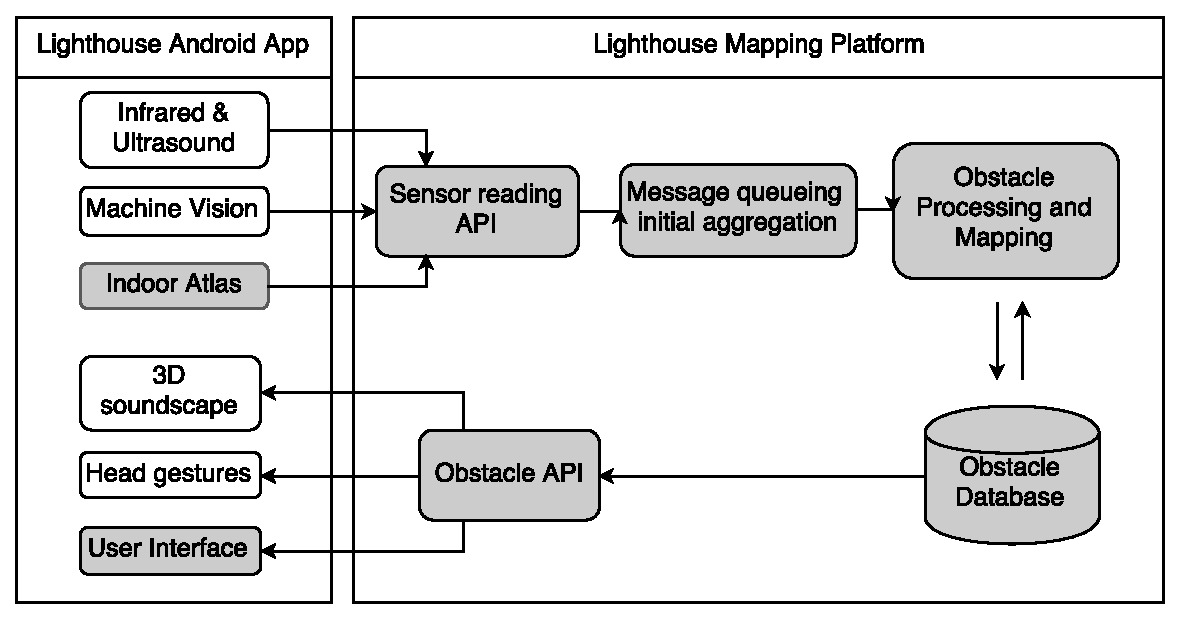
\includegraphics[width=\textwidth]{ReportDiagram.pdf}
\caption{System architecture}
\end{figure}

\subsection{Interactions}
\label{sec:interactions}
To facilitate communication between the server side and the client side the SSE team developed a portable library that handled the communication. It defines a clearly documented API for the use of the data collection and feedback applications. The library contains methods to synchronously or asynchronously send sensor readings to the data collection platform in addition to providing an API that allows the feedback applications to query the mapping platform for obstacles in an area. Each of the applications discussed in this section use these APIs to interact with the server side platform.

\subsection{Data collection and feedback}
The client side section of the project had two main jobs, one was to gather data from the sensors and relay them to the backend for further processing. The second is to give the user feedback on possible obstacles in the area and respond to commands from the user. Two of the sub components were the responsibility of the SSE team and each of the rest would be handled by a member of the CS team. This was done as a means to decouple the work of the CS students from the work of the SSE team and remove the SSE teams dependency on the work of the CS team. By having one data collection application and one feedback application developed by the SSE team and the rest by the CS team the risk to the SSE project was therefore reduced, in the event of the CS team not being able to finish their parts of the architecture.Most visually impaired people use IOS devices. However, for the data collection application we decided to use android application due to the fact that all members of the team are familiar with Java and have the required hardware to program on.

\subsubsection{Indoor Atlas location and obstacle listing}
The components developed by the SSE team were chosen so that a full slice of the system would be developed by the SSE team and any deliverables by the CS team would be additive. The app loads a map on to the screen of the mobile device and shows a point that represents the users location and heading.

The Indoor Atlas application uses an SDK developed by Indoor Atlas Ltd. \cite{IndoorAtlas} which uses magnetometric, accelerometer and gyroscopic sensors in a mobile device to determine a users location and heading indoors. In addition to sending the data to the server side the app also queries the server for the locations of obstacles. These obstacles are also drawn on the on-screen map.

\subsubsection{Visual obstacle detection}
The visual obstacle detection component uses a head mounted camera that takes pictures of the area in front of the user and uses a color detection algorithm to detect the floor area. Once the floor area is detected any obstacles of a different color are then detected and their location is sent to the data collection platform.

\subsubsection{Ultrasound and Infrared}
The ultrasound and infrared component also makes measurements of the objects in front of the user and send the readings to the obstacle mapping platform.
These measurements are done by using two infrared sensors and ultrasound sensor to detect the distance from the user to an obstacle. The three sensors readings are preprocessed and filtered to mitigate the effects of temperature, velocity and other factors before being sent to the data collection platform. 

\subsubsection{3D audio training}
The 3D audio training application leads a user through a series of steps that play sounds at certain bearings around the user. When the users hear the sound they turn their head so that they are facing the direction they think the sound is coming from. If the users are facing the correct direction they will be rewarded with a positive audible queue. If they are not they will get instructions on whether they are off to the left or right of the correct bearing. The application then gives the users a performance score which the users can then try to improve over time.

\subsubsection{Head gesture recognition}
\textcolor{orange}{Coming soon!!!}

\subsection{Obstacle processing and mapping}
The ultrasound, infrared and visual sensors are the minimal set of sensors decided upon for the initial iteration of the project, however the mapping platform was designed to accept any type of sensor reading. Therefore there are a few preprocessing steps between the data collection API described in section~\ref{sec:interactions} and the final obstacle processing and storage. A figure depicting the processing pipeline can be found in Appendix~\ref{app:SparkPipeline}.

\subsubsection{Data collection API}
The first point of contact in the data collection platform is the API mentioned in section~\ref{sec:interactions}. The responsibility of this component is to provide an interface for the server side that allows the data collection applications to send data to the server side platform. This is implemented by a server that listens on a UDP socket for messages in a specific JSON format. Once a message is received the message is validated and partially deserialised into a data structure and given a timestamp. The ID of the device sending the measurements is also recorded to allow the platform to correlate messages from different sensors from the same device.
%TODO: citation needed

\subsubsection{Aggregation}
\label{sec:aggregation}
After being partially deserialised the messages are filtered and split into categories. This step is designed so that the initial aggregation layer recognises the types of sensors and can map them to types that are used in the calculation of obstacles further down the pipeline. This allows for specific handling of each type of sensor in the aggregation layer while providing structured data down the line for processing. In the initial iteration there are three main data types, location, heading and distance. These sensor values are a minimum set necessary to infer the location of an obstacle based on a users location, heading and the distance to the obstacle. By abstracting the sensor values into these types the final obstacle calculations can be decoupled from the complexity of processing raw sensor readings and can be made more flexible. Once a sensor reading has been categorised it is pushed into a single message queue that is a part of a producer-consumer pattern. The producer-consumer pattern is implemented by the Apache Kafka message broker system~\cite{ApacheKafka}. Kafka provides a distributed messaging systems that allows for separation of large volumes of data into categorised streams called ``topics". This is used by the system to sort the deserialised data structures into topics which are then processed further.

\subsubsection{Processing and Mapping}
The readings produced and pushed into the Kafka topic in the step described in section~\ref{sec:aggregation} are consumed by a consumer that is implemented in Apache Spark~\cite{ApacheSpark}. Spark is a high performance, in memory, cluster computing framework. It provides a scalable platform that is capable of efficiently computing the large amount of data that the data collection applications can output. Spark Streaming is then used on top of the Spark processing platform to process the streamed topics provided by Kafka~\cite{ApacheSparkStreaming}.

In spark the categorised and partially deserialised sensor readings are fully serialised into concrete data types and then pushed into separate streams, one for location and heading and another for distance readings. This separation is to facilitate the preprocessing and filtering done in the next step. 

Once the streams have been separated based on data type the first pass of sensor fusion is performed. There is a moving average performed over each of the streams and an aggregation done to down sample the stream to a tick rate of 100ms. This smooths out noise in the sensor signal and gives a more accurate reading for each tick, which is then fed to the mapping calculation step.

Before performing the final mapping calculation the streams are joined and aligned based on the timestamp of the sensor reading and the ID of the device that performed the reading. This is done so that the mapping calculation can draw batches of measurements from each device over a certain time interval for further calculations. The result is a stream of sensor readings that is keyed by the server tick time and grouped by device id.

The last step involves a second pass of sensor fusion that consumes batches of readings from the joined stream and passes them through a calculation that extrapolates an obstacles position from a users location, heading and the distance measured by the sensors. These obstacles are then persisted in Apache Cassandra~\cite{ApacheCassandra}.

\subsubsection{Storage and obstacle API}
Cassandra is a highly performant, distributed NoSQL database that offers the same throughput and scalability as the other Apache products discussed in previous sections. The obstacles identified by the processing pipeline are stored in a table that contains the location, confidence and ID of an obstacle.

The feedback applications can then query Cassandra for obstacles by calling the Obstacle API. This API is a REST web service written in Java that queries the table in Cassandra and exposes a simple interface to the feedback applications.


\subsection{Testing strategy}
To test if the quality of the Lighthouse project meets the standard of the client, testing procedures were designed and implemented throughout the platform. Since different components of the architecture have different feature to test, unit, load and integration tests were implemented separately.

\subsubsection{Tools and Data generation}
The data was generated through a simulation script written in Python. The simulation was set up by specifying an agent, some obstacles and a set of sensors. The agent and obstacles would have a location in space and the agent had a maximum velocity, rotation speed and other movement parameters. The simulation would then be configured by laying out a path for the agent to move through while the sensors were polled to check if they would detect an obstacle. The simulation allowed for noise to be added to the sensor readings that would give a more realistic way of processing sensor data that will inherently contain error and noise.

\subsubsection{Unit testing}
Unit testing was used for Obstacle API which had several logic components. Each piece of logic was tested with actual data independently to assure that the output was as expected. The unit tests were run after each push to the Git repostitory through the Jenkins continous integration platform.


\subsubsection{Load testing}
After implementing the processing pipeline the first performance test performed was to evaluate the throughput and packet loss. This was done by sending progressively larger numbers of simulated sensor readings to the pipeline and measure how it handled the load.

\subsubsection{Integration testing}
Since the dependency of the processing component on the Spark environment creates  problems to unit testing, integration tests were found to be sufficient to assure the team that the processing is producing the correct results when the unit testing is hard to perform. Integration tests were performed by sending a simulated scenario of sensor readings through the processing pipeline to evaluate the obstacle detection accuracy. The simulated output was varied with respect to samling frequency, data rate and noise in the signal.

\subsubsection{Detection accuracy}
Describe the testing scenario, the simulator and show diagrams that compare both.
\textcolor{orange}{More to come}


\section{Evaluation}
Given the nature of the project the main success criteria is if the system can accurately determine the location of an obstacle in space based on the sensor data given. The evaluation of this fact was done by performing experiments with the actual sensor hardware, extracting the noise level, accuracy and other quality metrics and then generating sensor output based on those metrics. This generation of test data allowed us to evaluate the accuracy of our system in a controlled environment. We evaluated the robustness of our processing methods by increasing the noise in the generated sensor signal in addition to controlling the rate of data sent to the system. The throughput of the system was also evaluated by sending large amounts of sensor readings at a time and measuring response time, packet loss and transmission delay.

\subsection{Load testing}

\begin{center}
\begin{tabularx}{\textwidth}{| X | X | X | X |} 
\hline
\# Readings & Transmission time & \# Readings/Second & Packet Loss \% \\
\hline
7400 & 2.220366535 & 3332.783071 & 1.135135135 \\
\hline
74000 & 15.81466027 & 4678.380612 & 0.7731087894 \\
\hline
740000 & 119.9508543 & 5738.18339 & 5.847595525 \\
\hline
\end{tabularx}
\label{tab:performance}
\end{center}
%TODO: Label and reference the table

The results shown in table~\ref{tab:performance} show that the pipeline handled loads far beyond what was stipulated in the quality requirements, the packet loss is within acceptable limits (2\%) for over 100000 readings and the throughput was an order of magnitude higher than the goal. The quality requirements needed the pipeline to handle 100 readings per second but the load testing showed that the pipeline could handle over 5000 messages before it started to experience deteriorating performance.

\subsection{Integration testing}
Results show that the sensor fusion performed on the input manages to mitigate the noise up to a limit and provides much better results than when the processing pipeline is run without fusion.

\begin{center}
\begin{tabularx}{\textwidth}{| X | X | X | X |} 
\hline
No noise & No noise  & High noise  & High noise  \\
whithout fusion & with fusion & without fusion & with fusion \\
\hline
0.3849913005m & 0.3951750923m & 6.552494911m & 0.8089400658m \\
\hline
%0.2291972724m & 0.2288306005m & 23.88570995m & 1.465448725m \\
\hline
\end{tabularx}
\label{tab:performance}
\end{center}

%TODO: Talk about the cs students evaluation?
\subsection{Unit testing}




\section{Challenges and Lessons Learnt}
\subsection{Initially Proposed System}
\label{sec:Prelim}
%TODO: citation 
The initial plan for this project was to make use of device developed by students in the Electrical Engineering department. The hardware consists of an armband that can detect ultrasonic frequencies. Those frequencies are emitted by at least three beacons in strategically predefined locations in the room. The armband, in conjunction with a computer and an Android device, then triangulates the position of the armband in space.
The former use cases to be explored focused on detecting gestures and possible indoor location possibilities. However, soon after the project was presented to the team, the hardware was found to have several limitations. The team found that the location accuracy was considerably less than initially described. The initial description of the hardware stated that the location accuracy was sub-centimetre, which is the theoretical minimum, but the functional accuracy was between 10 and 50 centimetres. This eliminates the gesture use case since more precision is needed to get accurate gesture recognition.
%TODO: citation
Furthermore, the hardware can only function if three beacons are within a 130\degree cone in front of the receiver. This severely limits the practicality of the device for indoor location since a wearable piece of hardware is usually blocked by the wearer's body in addition to any obstacle in the environment such as static or movable objects.
%TODO: citation
Therefore the high probability of getting unacceptable performance out of the hardware platform was found to cause too much risk to the project and the team mitigated that risk by pivoting the focus of the project to a different topic.

\subsection{Testing with Real Data}
Despite creation of a program which simulates a user who moves in an environment full of obstacles, it is complicated to infer the accuracy of the platform based on simulated data. This is because the real data was expected to be provided by the CS students and it could differ from the data provided by the simulator. The challenge was that the CS student could provide real data only during the last few week of the project which gave us little time to test our platform with real data. 

\subsection{Memory Shortage}
Initially we rented a private server with only 2GB of main memory to run Oracle Java, Scala, Jenkins, Spark, Kafka, Zookeeper, Tomcat and Cassandra. These tools have high memory requirements, which the team underestimated. This caused runtime interuptions during development that required immediate remediation. 

To remedy these problems the team upgraded it's VPS subscription to a machine with 6GB of main memory and 25GB of secondary memory. Furthermore, allocating swap space of 6GB helped deal with any future memory issues. Lastly we set the machine to depend highly on main memory in order to keep I/O operations as fast as possible.

This situation had been avoidable if a thorough evaluation of the hardware requirements of all the technologies had been made in the early weeks of development.

\subsection{Shared communication library}
As described above a library was provided to the CS students which let them interact with our platform. Initially, we decided to implement this library on a desktop computer using Java 8. However, when we tried to use the library to send data to our platform we realised that android has several limitations on how it performs networking tasks. Specifically, it would not let to send data over socket on the main thread. Therefore, we had to re-implement the library to be compatible with android devices. The effect of this problem was slightly mitigated by the fact the SSE team developed one of the data collection applications, this meant that the testing of the library could be done fully by the SSE team without having to send it to the CS students for testing.

\subsection{Java over Scala for Spark}
As described above it was decided to use Java as a programming language for Spark processing. Making this decision led us to several challenges which we couldn't know beforehand. First, despite that there was plenty of Java code documentation we still spent a lot of time on implementing the required features. That is due to the fact that the official Java code was not working anymore with the latest Spark version because of methods deprecation. Therefore, we were forced to learn the technology more deeply in order to workaround these problem. 

From the experience with Spark programming we have learned that sometimes it is better to learn a new language for which the technology was initially implemented instead of picking an already familiar language in order to program on the new technology. In addition, the code would be much cleaner if we had used Scala instead of Java.

\subsection{Combining Data Streams}
Another challenge, on top of absence of up-to-date documentation, was understanding how Spark is processing data and how to write code for it. Initially the sensor data processing was written in standard Java 8. We encountered several problems when tried to integrate the code into Spark since it uses different concept of data, where data stream contains batches of sensor data. First, Spark didn't let us to work with sensor data in different batches as we expected. Therefore, we had to completely change the processing approach, which also took us time.

The experience was helpful to understand that implementation of features should be right away done for the technology which is going to be used.

\subsection{Cassandra Data Modelling}
\textcolor{orange}{Lots to say here, see if we have space}

\section{Life cycle and Future Work}
\subsection{Current state}
\label{sec:current}
The Lighthouse project now can process data from two kinds of sensors, location and rangefinding sensors, and achieves the aim of detecting obstacles through the use of them. The project reaches the goal of using low-cost and off-the-shelf sensors. Currently, the magnetic sensor in the android device, camera, Infrared and Ultrasound sensors work together to collect data from the indoor environment and send all the information collected to data processing component by implementing the API created by SSE team. After the processing, feedback will be shown to users in map and 3D sound. The two most important factor of performance are latency and accuracy. In our testing mentioned above, the quality of the project can fulfill the requirement of indoor real-time obstacle detection.
\textcolor{orange}{(need to add some testing result)}

\subsection{Future work}

\subsubsection{Cluster computing}
As described in~\ref{sec:current}, all the data from the previously mentioned sensors are queued and process by a single machine. Looking into the future were more sensors would be attached to the client's device and a possible staggering number of active users, it would be of high importance to scale out our current system to meet future compuational demands. The benefit of deploying kafka, Zookeeper, Spark and Cassandra as part of our solutuion is they were all built to be used in a distributed environment hence making scaling out a less tedious. Cluster computing will guarantee fault tolerance to our data collection platform and higher computational speed for our running processes.

\subsubsection{Sensor fusion}

\subsubsection{NoSQL to MySQL}

\subsection{Maintenance and Scaling}
% TODO: Enumerate limitation of the product
% TODO: Describe how we can go from prototype to a running system
In the future, when the project needs to be expanded with other types of sensors, this platform can still provide the interface for communication between device and processing component. 
Although this product can fulfil the client's requirements, it has huge performance disparity with a real industry product. Since budget and experience are limited, the capability of the project is not sufficient to support thousands of simultaneous user queries at the moment.

This project can be migrated to Azure which is a Microsoft product and can provide global coverage and high availability and stability. The components of the project need to be rewritten in C\# and Azure analog technologies. Please refer to Appendix~\cite{app:MigrationPlan} for a detailed description of a possible migration strategy.


\section{Conclusion}
Moving around without others’ assistance in an unfamiliar environment is always a challenge for the visually impaired especially in a place where the obstacles are changing. To solve this problem, the Lighthouse team managed to deliver a product which consists of data collection component with sensors, data processing platform and feedback component build in Android. The sensors which include the magnetic sensor in Android phone, infrared sensor, ultrasound sensor and camera collected data of environment and sent them to processing platform via Kafka. After processing, the Android application showed the details of surroundings to users. In testing, each component in this project showed satisfied quality which met most of the requirements from stakeholders. 

Both Microsoft and the visually impaired people can benefit from the Lighthouse project. First, it can help Microsoft enlarge the market for the visually impaired since there is an enormous amount of people living with sight loss. Second, the Lighthouse project provides a prototype which is both low-cost and easy to deploy to help Microsoft economise the funds. Also, for visually impaired users, the Lighthouse project not only assist them get details of surroundings but also enrich their confidence to explore the world on their own. 


% TODO: identify the topic takeaway messages.
% takeaway messages describe how we one could do things differently.
% not in context of the project but rather in the context of the domain. 

% Appendix
\appendix
\section*{APPENDIX} \label{Appendix}
\setcounter{section}{1}

\appendixhead{ZHOU}

% Acknowledgments
\begin{acks}
\end{acks}  

% Bibliography
\bibliographystyle{ACM-Reference-Format-Journals}
\bibliography{GroupReport-bibfile}

% History dates
%\received{February 2007}{March 2009}{June 2009}

% Electronic Appendix
\elecappendix

\medskip

\section{Migration plan}
\label{app:MigrationPlan}
\section{This is an example of Appendix section head}

\pagebreak
\section{Spark Pipeline Figure}
\label{app:SparkPipeline}
\begin{figure}[!ht]
\label{fig:SparkPipeline}
\centering
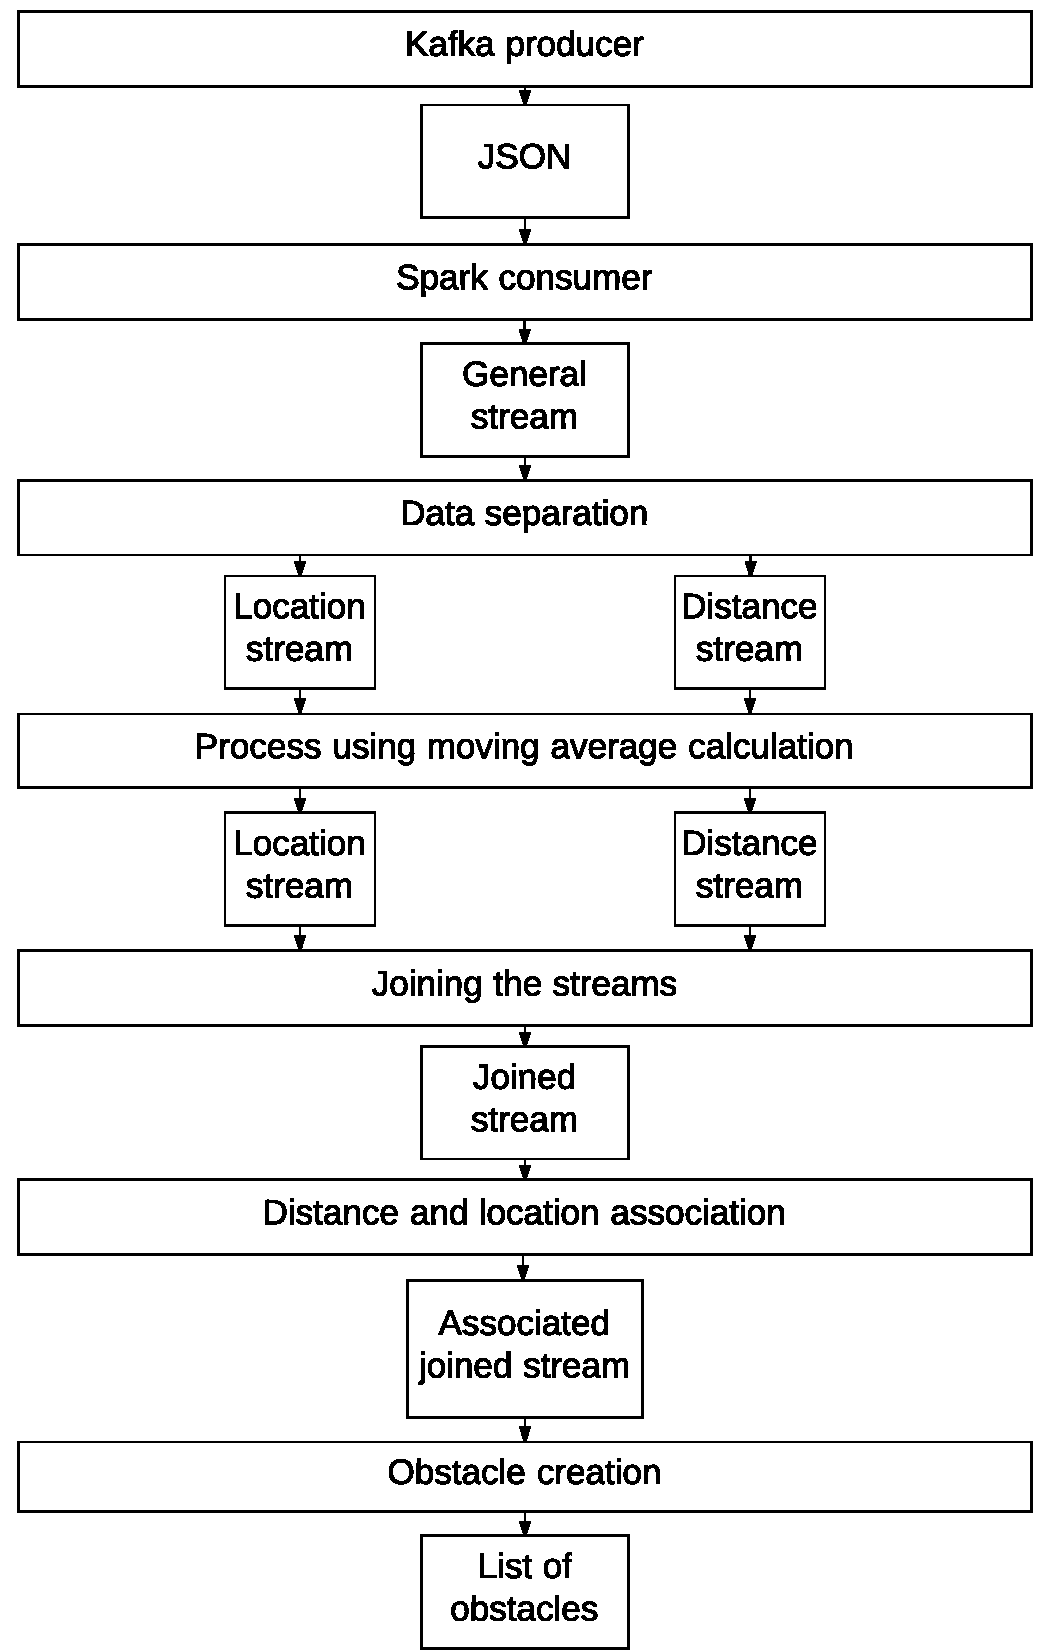
\includegraphics[width=0.8\textwidth]{SparkPipeline.pdf}
\caption{Spark processing pipeline}
\end{figure}
\clearpage
\pagebreak
\section{Architecture cost analysis}
\label{ArchitectureCost}

\section{Requirements}
\begin{center}
\begin{tabularx}{\textwidth}{| X | X |} 
 \hline
 \rowcolor{lightgray}
 \multicolumn{2}{|c|}{List of Requirements} \\ [0.5ex] 
 \hline\hline
 Identifying points of interest in the environment. &  Detecting obstacles \\
 \hline
 Feeding back mapping information &  Manually identifying obstacles in a space \\
 \hline
 Manually removing an obstacle from the map &  Providing navigation for a user to a point of interest \\ 
 \hline
 Voice interactions - listing &  Voice interactions - acceptance \\ 
 \hline
 Screen interactions - listing &  Screen interactions - acceptance \\ 
 \hline
 Classification of obstacles/Points Of Interest &  3D Directional Sound \\ 
 \hline
 Head Gestures &  IR and Ultrasound \\  
 \hline

 \hline
\end{tabularx}
\label{tab:requirements}
\end{center}
\end{document}



